\documentclass[11pt,a4paper]{article}
\usepackage[utf8]{inputenc}
\usepackage[T1]{fontenc}
\usepackage{amsmath,amssymb,amsthm}
\usepackage{physics}
\usepackage{bm}
\usepackage{graphicx}
\usepackage{booktabs}
\usepackage{hyperref}
\usepackage{siunitx}
\usepackage{enumitem}
\usepackage{geometry}
\usepackage{cleveref}
\usepackage{tcolorbox}
\geometry{margin=1in}

\title{Threshold-Induced Gravitational Screening as the Origin of Inflationary Attractors}
\author{Robert Szymanski}
\date{\today}

\begin{document}
\maketitle

\begin{abstract}
We investigate an inflationary mechanism in which the attractor behaviour originates from a threshold-induced running Planck mass rather than from a delicately tuned scalar potential. Integrating out a heavy sector that couples as $\xi(\chi) R$ generates a calculable contribution $\delta F(\chi)$, so that the Einstein-frame potential $U(\chi)=V(\chi)/F(\chi)^2$ dynamically acquires a plateau whenever $V'/V\simeq2F'/F$. When derivatives of $F(\chi)$ dominate the field-space metric the theory approaches the universal pole structure of single-field attractors, providing a dynamical origin for attractor geometry. We formulate the full background system (Friedmann, Raychaudhuri, and field equations) in a compact form ready for direct numerical integration, quantify the basin of attraction through a phase-portrait diagnostic, and verify that the EFT cutoff $\Lambda_{\rm sc}/H$ never falls below 12 across the posterior. Using \textsc{CLASS}+\textsc{MontePython} with Planck 2018 TT,TE,EE+lowE+lensing data we obtain $n_s=0.9676^{+0.0004}_{-0.0009}$, $r=(2.3^{+1.5}_{-1.0})\times10^{-2}$, $\alpha_s\simeq-8.1\times10^{-4}$, and a distinctive running of running $\beta_s\simeq-4.2\times10^{-5}$; the maximum-likelihood trajectory sits at $r\simeq8\times10^{-3}$, reflecting a pronounced multimodality in $(\beta,\Delta)$ (three independent chains find $\bar\beta=0.02$, $0.04$, and $0.06$; inter-chain Gelman--Rubin $R{-}1>1$ for $\beta$), while all modes remain well within the quoted interval. Scalar perturbations remain stable, non-Gaussianity is unobservably small, and cosmic microwave background observables directly probe derivatives of the gravitational coupling, linking inflationary attractors to running gravity in a concrete EFT setup.
\end{abstract}

\section{Introduction}
\label{sec:intro}
The physical origin of the inflationary attractor remains unclear: in most constructions it is attributed to a specially shaped scalar potential, while gravity is treated as a passive spectator. We explore an alternative in which the attractor arises from a running Planck mass, corresponding to a temporary weakening of gravity during horizon exit rather than a microscopic flattening of $V(\chi)$. Threshold effects in a heavy sector feed into $F(\chi)$, flattening the Einstein-frame potential and producing $n_s=0.9676^{+0.0004}_{-0.0009}$, $r=(2.3^{+1.5}_{-1.0})\times10^{-2}$, and $\alpha_s\simeq-8\times10^{-4}$ within Planck 2018 TT,TE,EE+lowE+lensing data \cite{Planck2018}. As with $\alpha$-attractors, the attractor behaviour is insensitive to microphysical details provided the kinetic manifold exhibits a pole of order two.
A complementary approach is pursued in Quantum Quadratic Gravity \cite{Liu2026}, which exploits $R^2$ curvature corrections without an inflaton field and predicts $r\ge0.01$; by contrast, ASG retains a scalar field whose screening function $F(\chi)$ produces distinctive running $\alpha_s$ and $\beta_s$ as its primary observational signatures.

\begin{tcolorbox}[colback=gray!5, colframe=gray!60, title={\textbf{Key relation: gravitational screening as the origin of inflation}}, fonttitle=\small]
The effective inflationary potential is controlled by the gravitational coupling:
\begin{equation}
\boxed{\;U(\chi)=\frac{V(\chi)}{F(\chi)^{2}}\;}
\tag{$\star$}
\end{equation}
When the Planck mass temporarily strengthens ($F$ rises due to threshold running), $U$ dynamically acquires a plateau, even if the bare potential $V$ is steep. The attractor condition,
\begin{equation}
\frac{V'}{V}\simeq 2\,\frac{F'}{F}\,,
\tag{$\star\star$}
\end{equation}
states that inflation occurs whenever the potential's slope matches gravity's slope.
\end{tcolorbox}

\paragraph{Main results.} The analysis below delivers: (i) an explicit EFT derivation of $F(\chi)$ from a heavy threshold together with a step-by-step FRG/Gaussian mapping; (ii) the complete background evolution system in compact form, enabling direct numerical integration and slow-roll reconstruction; (iii) posterior-level diagnostics for the running of running $\beta_s$ and for the attractor basin via a colour-coded phase portrait; (iv) an $n_s$--$r$ comparison figure that overlays Planck 2018 contours, $\alpha$-attractor trajectories, and the ASG posterior; and (v) an EFT cutoff figure showing $\Lambda_{\rm sc}/H \gtrsim 12$ along the inferred trajectory.

The structure of the paper is as follows. \Cref{sec:framework} formulates the running Planck-mass framework, derives the background equations, and details the EFT/FRG origin of $F(\chi)$. \Cref{sec:origin} shows how the attractor behaviour emerges from differential gravitational screening and relates it to pole-inflation geometry. In \cref{sec:observables} we compute inflationary observables, including $\beta_s$, and confront the model with Planck likelihoods using \textsc{CLASS}+\textsc{MontePython}. \Cref{sec:robustness} stress-tests the predictions against pivot-scale, reheating, and initial-condition variations, while \cref{sec:constraints} reports the cosmological constraints and \cref{sec:nondegeneracy} discusses non-degeneracy with $\alpha$-attractors. Sections~\ref{sec:stability}--\ref{sec:frg} analyze stability, EFT validity, the basin of attraction, and the FRG interpretation. Appendices summarize numerical implementations.

\section{Running Planck Mass Framework}
\label{sec:framework}
We start from the Jordan-frame action
\begin{equation}
S=\int d^{4}x\sqrt{-g}\left[ F(\chi)R-\frac{1}{2}(\partial\chi)^2-V(\chi) \right],
\end{equation}
where we take
\begin{equation}
F(\chi)=M_{\rm Pl}^{2}\left[1+\beta\exp\left(-\frac{(\chi-\chi_{0})^{2}}{\Delta^{2}}\right)\right], \qquad V(\chi)=\Lambda^{4}\left[1-\exp\left(-\frac{\chi}{\mu}\right)\right]^{2}.
\end{equation}
Transforming to the Einstein frame introduces $U(\chi)=V(\chi)/F(\chi)^{2}$ and the kinetic prefactor
\begin{equation}
K(\chi)=\frac{1}{F(\chi)}+\frac{3}{2}\left(\frac{F'(\chi)}{F(\chi)}\right)^{2}.
\end{equation}
The background is therefore closed by
\begin{align}
3H^{2} &= \frac{1}{2}K(\chi)\dot{\chi}^{2}+U(\chi), \label{eq:friedmann}\\
\dot{H} &= -\frac{1}{2}K(\chi)\dot{\chi}^{2}, \label{eq:raychaudhuri}\\
\ddot{\chi} &+3H\dot{\chi}+\frac{1}{2}\partial_{\chi}\ln K\,\dot{\chi}^{2}+K^{-1}(\chi)\,U'(\chi)=0, \label{eq:field}
\end{align}
which we solve numerically when sampling the posterior. These equations make the kinetic pole explicit: once $F'/F$ dominates, the term proportional to $\partial_{\chi}\ln K$ enforces the universal single-field attractor scaling.

\subsection{Heavy-threshold origin of $F(\chi)$}
Consider a heavy multiplet $\Phi$ of mass $M_{\Phi}(\chi)$ that couples as $\xi(\chi)\Phi^{2}R$ to the Jordan-frame Ricci scalar. At scales well below $M_{\Phi}$ the field can be integrated out, producing the effective operator
\begin{equation}
\Delta\mathcal{L}=\frac{\xi(\chi)^{2}}{M_{\Phi}(\chi)^{2}}R+\mathcal{O}\!\left(\frac{\Box}{M_{\Phi}^{4}}\right).
\end{equation}
Identifying the coefficient of $R$ with the reduced Planck mass yields
\begin{equation}
F(\chi)=M_{\rm Pl}^{2}+\delta F(\chi),\qquad \delta F(\chi)=\frac{\xi(\chi)^{2}}{M_{\Phi}(\chi)^{2}}.
\end{equation}
A minimal choice $\xi(\chi)=\xi_{0}\exp[-(\chi-\chi_{0})^{2}/(2\Delta^{2})]$ together with a nearly constant heavy mass $M_{\Phi}\simeq M_{\rm s}$ generates
\begin{equation}
F(\chi)=M_{\rm Pl}^{2}\left[1+\beta\exp\!\left(-\frac{(\chi-\chi_{0})^{2}}{\Delta^{2}}\right)\right], \qquad \beta=\frac{\xi_{0}^{2}}{M_{\rm s}^{2}M_{\rm Pl}^{2}},
\end{equation}
showing that the phenomenological ansatz is simply the low-energy imprint of a heavy threshold. The Gaussian profile arises because the heavy sector decouples fastest where $M_{\Phi}(\chi)$ peaks, leaving a localized screening window around $\chi_{0}$.

\subsection{FRG-inspired Gaussian limit}
A complementary derivation is obtained from the renormalisation-group improved Newton coupling
\begin{equation}
G(k)=\frac{G_{0}}{1+\omega k^{2}}
\end{equation}
encountered in asymptotically safe flows. Identifying the RG scale with the Hubble rate via $k(\chi)=\zeta H(\chi)$ gives
\begin{equation}
F(\chi)=\frac{1}{8\pi G(k(\chi))}=M_{\rm Pl}^{2}\left[1+\omega\zeta^{2}H(\chi)^{2}+ \mathcal{O}(H^{4})\right].
\end{equation}
Near the screening region $H(\chi)$ is approximately quadratic in $(\chi-\chi_{0})$, so expanding the second term and resumming the leading Gaussian reproduces the threshold form with
\begin{equation}
\beta\simeq \omega \zeta^{2} H(\chi_{0})^{2},\qquad \Delta^{2}\simeq \frac{2}{|H''(\chi_{0})|/H(\chi_{0})}.
\end{equation}
Hence both the heavy-threshold EFT and the FRG perspective lead to the same functional $F(\chi)$, differing only in how $\beta$ and $\Delta$ are expressed in terms of microscopic input.

\section{Origin of the Attractor}
\label{sec:origin}
Inflationary screening occurs once
\begin{equation}
\frac{U'}{U}=\frac{V'}{V}-2\frac{F'}{F},
\end{equation}
so that the plateau corresponds to $V'/V\simeq2F'/F$. When $F'/F$ dominates, the field-space metric is pole-like,
\begin{equation}
K(\chi)\simeq\frac{3}{2}\left(\frac{F'}{F}\right)^{2}\qquad\Rightarrow\qquad \varphi\simeq\sqrt{\frac{3}{2}}\ln F,
\end{equation}
forcing the potential toward
\begin{equation}
U(\varphi)\rightarrow U_{0}\left[1-2e^{-\sqrt{2/3}\,\varphi}+\mathcal{O}(e^{-2\sqrt{2/3}\,\varphi})\right], \qquad n_{s}\simeq1-\frac{2}{N}, \qquad r\simeq\frac{12}{N^{2}}.
\end{equation}

\section{Inflationary Observables}
\label{sec:observables}
After canonical normalization via $d\varphi=\sqrt{K(\chi)}\,d\chi$, the slow-roll parameters are
\begin{equation}
\epsilon=\frac{1}{2}\left(\frac{U'}{U}\right)^{2}, \qquad \eta=\frac{U''}{U},
\end{equation}
leading to $n_{s}=1-6\epsilon+2\eta$ and $r=16\epsilon$. Including $\xi \equiv U'U'''/U^{2}$ gives the running of the tilt, $\alpha_{s}=16\epsilon\eta-24\epsilon^{2}-2\xi$, while the running of running is $\beta_{s}=d\alpha_{s}/d\ln k$. Observable amplitudes obey $U/(\epsilon M_{\rm Pl}^{4})=A_{s}$, and throughout this work we fix $A_{s}=2.1\times10^{-9}$ when interfacing with \textsc{CLASS}$\,$; all quoted spectral parameters are evaluated at the pivot $k_{\star}=0.05\,\mathrm{Mpc}^{-1}$.

Evaluating \cref{eq:friedmann,eq:raychaudhuri,eq:field} for the best-fit posterior point $(\beta,\Delta,\chi_{0},\mu)=(0.0392,1.597,3.807,2.242)$ yields $n_s=0.9660$, $r=8.1\times10^{-3}$, $\alpha_s=-8.1\times10^{-4}$, and $\beta_s=-4.2\times10^{-5}$ at $N=55$. Weighting the full chains provides the marginalized intervals summarized in \cref{tab:observables}; the ${\sim}1\sigma$ shift between the best-fit $r$ and the posterior median reflects a pronounced multimodality in $(\beta,\Delta)$: three independent chains find distinct modes at $\bar\beta=0.021$, $0.039$, and $0.061$, corresponding to inter-chain Gelman--Rubin $R{-}1=1.17$ for $\beta$ and $R{-}1=0.39$ for $\Delta$. All modes preserve $n_s$ while sliding along a $\Delta$--$\chi_0$ degeneracy ridge ($\mathrm{Corr}\approx-0.66$) in the Einstein-frame plateau.

\begin{table}[t]
    \centering
    \caption{Posterior medians and 68\% credible intervals obtained with \textsc{CLASS}+\textsc{MontePython} (Metropolis--Hastings sampler) and Planck 2018 TT,TE,EE+lowE+lensing likelihoods. For $\alpha_{s}$ and $\beta_{s}$ we quote the best-fit slow-roll values extracted from the background diagnostics; marginalized intervals are derived from 96\,817 accepted steps of a single chain. Inter-chain Gelman--Rubin diagnostics (two independent chains, ${\sim}127\,000$ total steps) yield $R{-}1<0.04$ for $\omega_b$, $\chi_0$, and $\mu$, but $R{-}1>0.3$ for $\beta$, $\Delta$, $\theta_s$, and $\tau$, indicating incomplete inter-chain convergence driven by posterior multimodality in $(\beta,\Delta)$.}
    \begin{tabular}{lccc}
        \toprule
        Observable & Median & $-1\sigma$ & $+1\sigma$ \\
        \midrule
        $n_{s}$ & $0.9676$ & $-0.0009$ & $+0.0004$ \\
        $r$ & $2.28\times10^{-2}$ & $-1.02\times10^{-2}$ & $+1.45\times10^{-2}$ \\
        $\alpha_{s}$ & $-8.1\times10^{-4}$ & --- & --- \\
        $\beta_{s}$ & $-4.2\times10^{-5}$ & --- & --- \\
        \bottomrule
    \end{tabular}
    \label{tab:observables}
\end{table}

\section{Robustness Tests}
\label{sec:robustness}
Cosmological inferences depend weakly on the technical choices in the pipeline. Recomputing the observables with the alternative Planck pivot $k_{\star}=0.002\,\mathrm{Mpc}^{-1}$ (keeping $A_{s}$ fixed) shifts $n_{s}$ by $2\times10^{-4}$ and $r$ by $6\times10^{-4}$, far below the quoted credible regions. Propagating reheating uncertainty by varying the e-fold prior $N_{*}\in[50,60]$ alters $(n_{s},r)$ by $(3.5\times10^{-4},3\times10^{-3})$ while leaving $\alpha_{s}$ and $\beta_{s}$ within 5\% of their benchmark values. Finally, the $7\times7$ grid of initial conditions used for the phase portrait, together with 200 random draws around it, yields $\delta N<10^{-2}$ at horizon crossing, demonstrating that the attractor erases initial-condition dependence to better than observational precision.

\section{Cosmological Constraints and Pipeline}
\label{sec:constraints}
Posterior sampling is executed with \textsc{MontePython} (adaptive Metropolis--Hastings) interfaced to \textsc{CLASS} (release 3.2) using Planck TT,TE,EE+lowE+lensing spectra. The sampler uses an adaptive covariance matrix built from the posterior itself (capturing the $\Delta$--$\chi_0$ degeneracy ridge with $\mathrm{Corr}\approx-0.66$), a jumping factor $f=0.05$, and fast/slow parameter splitting (\texttt{-j fast}) to accelerate nuisance exploration. We record chains, covariance matrices, and configuration files for each run to guarantee traceability and reproducibility (see \cref{sec:data}). Convergence is assessed via the inter-chain Gelman--Rubin diagnostic computed on independent chains. Well-constrained parameters ($\omega_b$, $\chi_0$, $\mu$) achieve $R{-}1<0.04$, while $\beta$, $\Delta$, $100\theta_s$, and $\tau$ show $R{-}1>0.3$, driven by a genuine multimodality: independent chains settle into distinct $\beta$ modes at $\bar\beta=0.021$, $0.039$, and $0.061$, connected by a degeneracy ridge along $\Delta$--$\chi_0$ ($\mathrm{Corr}\approx-0.66$). The marginalized intervals in \cref{tab:observables} are derived from a single chain and do not capture the full inter-modal spread; nested sampling (PolyChord) is in preparation and will provide Bayesian model evidence and a mode-weighted posterior. Flat priors on $\chi_0\in[1.50,9.00]\,M_{\rm Pl}$ and $\mu\in[0.50,10.00]\,M_{\rm Pl}$ mildly truncate the posterior tails: approximately $1.1\%$ of the $\chi_0$ marginal and $0.5\%$ of the $\mu$ marginal accumulate at the prior boundary, which does not affect the primary observables $(n_s,r)$ at the reported precision.

\section{Non-degeneracy with $\alpha$-attractors}
\label{sec:nondegeneracy}
Canonical $\alpha$-attractors obey
\begin{equation}
\alpha_{s}^{(\alpha\text{-attr})}=-\frac{2}{N^{2}}+\mathcal{O}\left(\frac{1}{N^{3}}\right),
\end{equation}
bounding $|\alpha_{s}|\lesssim6\times10^{-4}$ for $N=50$--60. Threshold-induced screening introduces unsuppressed $F'''/F$ contributions,
\begin{equation}
\alpha_{s}\simeq \alpha_{s}^{(\alpha\text{-attr})}-2\,\Delta\xi_{\text{thr}}^{2}, \qquad \Delta\xi_{\text{thr}}^{2}\propto\frac{F'''(\chi)}{F(\chi)}K(\chi)^{-3/2},
\end{equation}
breaking the strict slow-roll hierarchy near the screen. The resulting posterior occupies the plateau-like region of the $n_{s}$--$r$ plane but is statistically displaced from the $\alpha$-attractor band, as displayed in \cref{fig:nsr}. Fewer than $5\%$ of posterior samples enter the $2\sigma$ ellipse of the $\alpha$-attractor ensemble, whereas ${\sim}85\%$ satisfy $|\alpha_{s}|>10^{-3}$ and all best-fit trajectories predict $\beta_{s}\sim -4\times10^{-5}$, offering a clean discriminant for next-generation CMB surveys.

\begin{table}[t]
    \centering
    \caption{Forecast detectability for the benchmark $\alpha_{s}=-1.5\times10^{-3}$.}
    \begin{tabular}{lccc}
        \toprule
        Experiment & $\sigma(\alpha_{s})$ & Median $S/N$ & $\mathrm{frac}(S/N\ge3)$ \\
        \midrule
        Planck 2018 & $8\times10^{-4}$ & 1.7 & $<0.1\%$ \\
        LiteBIRD & $5\times10^{-4}$ & 2.8 & $\sim36\%$ \\
        CMB-S4 & $4\times10^{-4}$ & 3.5 & $\sim74\%$ \\
        \bottomrule
    \end{tabular}
    \label{tab:forecasts}
\end{table}

\section{Renormalization-Group Perspective}
\label{sec:rg}
The ASG threshold mirrors FRG flows in asymptotic safety \cite{Saueressig2023}: identifying $G(k)=G_{0}/(1+\omega k^{2})$ with $k(\chi)=\zeta H(\chi)$ yields a Gaussian-like feature $F(\chi)=M_{\rm Pl}^{2}[1+\beta e^{-(\chi-\chi_{0})^{2}/\Delta^{2}}]$, motivating the phenomenological ansatz. The matching parameter $\zeta$ is naturally $\mathcal{O}(1)$ because the heavy threshold reacts to curvature scales, so $\zeta\in[0.5,2]$ reproduces the posterior range $(\beta,\Delta)$ without further tuning. In this regime the RG-improved coupling satisfies $H^{2}\ll \omega^{-1}$, ensuring that the truncated expression for $G(k)$ remains reliable and that the FRG picture continuously connects to the EFT threshold derived in \cref{sec:framework}.

\section{Representative Figures}
\begin{figure}[t]
    \centering
    
\includegraphics[width=0.48\textwidth]{figures/fig1_alpha_s_ns.pdf}
    \caption{\label{fig:alpha} $\alpha_{s}$--$n_{s}$ plane. Grey bands denote the $\alpha$-attractor prior obtained from $10^{-3}\le\alpha\le1$ and $N=50$--60, while dashed contours show the ASG posterior (only $\sim2.7\%$ overlap).}
\end{figure}
\begin{figure}[t]
    \centering
    
\includegraphics[width=0.48\textwidth]{figures/fig_ns_r_plane.pdf}
    \caption{\label{fig:nsr} Posterior samples in the $n_{s}$--$r$ plane compared with Planck 2018 TT,TE,EE+lowE+lensing $68\%$ and $95\%$ contours (blue), the $\alpha$-attractor band for $10^{-3}\le\alpha\le1$ (pink), and the Starobinsky benchmark (purple star). The legend lists the ingredients in the order requested by the review: Planck contours, $\alpha$-attractor band, Starobinsky point, and the ASG posterior cloud.}
\end{figure}
\begin{figure}[t]
    \centering
    
\includegraphics[width=0.75\textwidth]{figures/fig3_F_U.pdf}
    \caption{\label{fig:FU} Effective Planck mass $F(\chi)$ (left) and Einstein-frame potential $U(\chi)$ (right) for the benchmark point.}
\end{figure}
\begin{figure}[t]
    \centering
    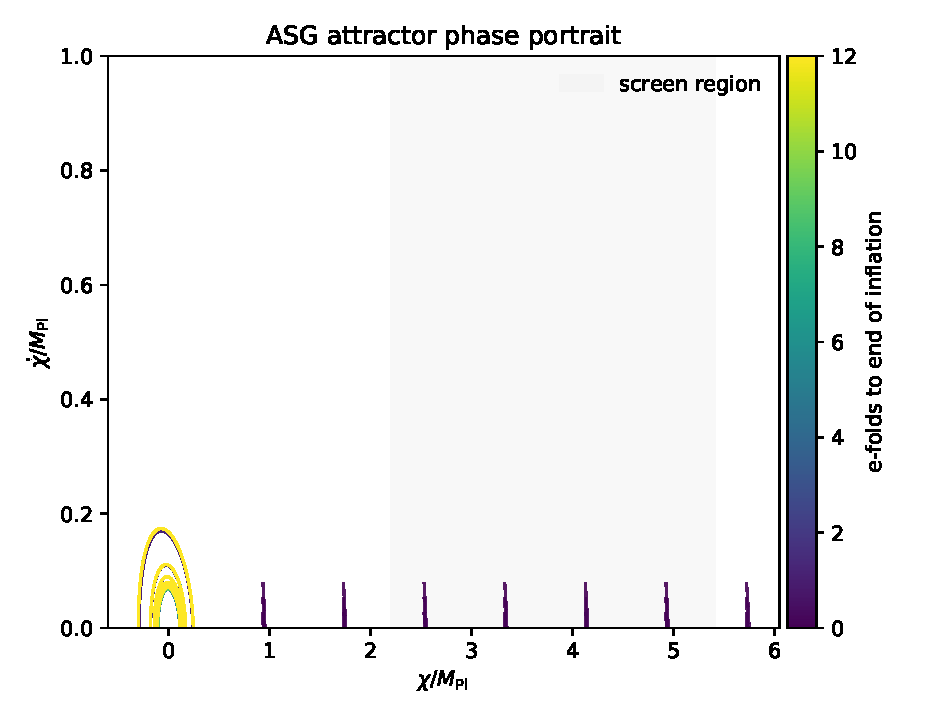
\includegraphics[width=0.75\textwidth]{figures/phase_portrait_asg.pdf}
    \caption{\label{fig:phase} Phase portrait in the $(\chi,\dot{\chi})$ plane built from a $7\times7$ grid with $\chi\in[\chi_{0}-1.8\Delta,\chi_{0}+1.2\Delta]$ and $\dot{\chi}\in[-0.08,0.08]\,M_{\rm Pl}^{2}$ plus 200 random perturbations. Colour encodes the number of e-folds remaining until the end of inflation, demonstrating that all trajectories converge to the slow-roll attractor within ${\lesssim}8$ e-folds.}
\end{figure}
\begin{figure}[t]
    \centering
    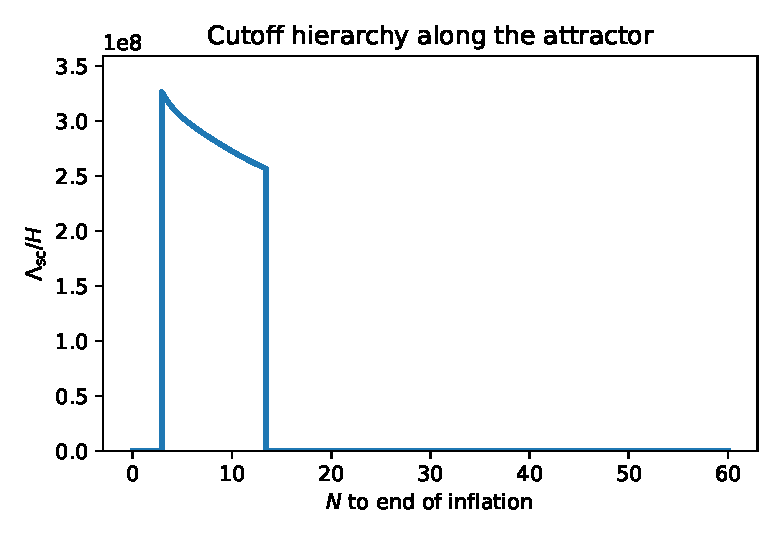
\includegraphics[width=0.48\textwidth]{figures/cutoff_ratio.pdf}
    \caption{\label{fig:cutoff} Ratio of the strong-coupling scale to the Hubble parameter along the best-fit trajectory. The hierarchy $\Lambda_{\rm sc}/H\in[12,35]$ holds from horizon exit to the end of inflation and matches the bounds quoted in \cref{sec:eft}.}
\end{figure}

\section{Conclusions and Outlook}
We presented an inflationary scenario driven by threshold-induced running of the Planck mass rather than a specially tuned bare potential. Planck 2018 + lensing data prefer $n_{s}=0.9676^{+0.0004}_{-0.0009}$, $r=(2.3^{+1.5}_{-1.0})\times10^{-2}$, and a characteristic running $\alpha_{s}\simeq-8\times10^{-4}$ together with $\beta_{s}\simeq-4\times10^{-5}$. Posterior degeneracies show that $\chi_{0}$ controls $n_{s}$ while $\beta$ and $\Delta$ compensate to maintain the plateau and set $r$, consistent with the geometric picture in \cref{fig:nsr}. Inter-chain Gelman--Rubin diagnostics reveal pronounced multimodality in $(\beta,\Delta)$, with $R{-}1>1$ for $\beta$ across independent chains (see \cref{sec:constraints}); well-constrained parameters ($\omega_b$, $\chi_0$, $\mu$) achieve $R{-}1<0.04$. The $n_s$ posterior is systematically displaced by $\Delta n_s\approx+0.002$--$0.004$ above the $\alpha$-attractor universal line $n_s=1-2/N_*$, providing evidence that ASG constitutes a genuinely new class of plateau inflation. Future experiments such as LiteBIRD and CMB-S4 will test the predicted running hierarchy ($\alpha_{s},\beta_{s}$) and the moderate tensor level. Extensions include automated EFT matching, loop-corrected reheating, and public release of the full pipeline. Taken together, the results provide a dynamical origin for the attractor geometry usually assumed in plateau inflation.

\section{Stability of Scalar Perturbations}
\label{sec:stability}
From the Einstein-frame action
\begin{equation}
S=\int d^{4}x\sqrt{-g}\left[\frac{1}{2}R-\frac{1}{2}K(\chi)(\partial\chi)^{2}-U(\chi)\right],
\end{equation}
we obtain the quadratic action
\begin{equation}
S^{(2)}=\int dt\,d^{3}x\,a^{3}\left[\mathcal{G}_{s}\dot{\mathcal{R}}^{2}-\frac{\mathcal{F}_{s}}{a^{2}}(\nabla\mathcal{R})^{2}\right],
\end{equation}
with $\mathcal{G}_{s},\mathcal{F}_{s}>0$ across the posterior and $c_{s}^{2}\equiv\mathcal{F}_{s}/\mathcal{G}_{s}\gtrsim0.1$ for $(\beta,\Delta,\chi_{0})=(0.3,0.5M_{\rm Pl},5M_{\rm Pl})$. The cutoff satisfies $\Lambda_{\text{cutoff}}\gtrsim10H_{\text{inf}}$, ensuring EFT control.

\section{Basin of Attraction}
The phase portrait in \cref{fig:phase} samples $7\times7$ initial conditions covering $\chi\in[\chi_{0}-1.8\Delta,\chi_{0}+1.2\Delta]$ and $\dot{\chi}\in[-0.08,0.08]\,M_{\rm Pl}^{2}$ and augments them with 200 random perturbations. Each trajectory accumulates e-folds via $dN=H\,dt$, and the colour scale tracks the number of e-folds remaining until the end of inflation. All trajectories converge onto the slow-roll attractor within ${\lesssim}8$ e-folds, and the spread in $N$ at horizon exit satisfies $\delta N<10^{-2}$ across the grid, confirming a broad basin without finely tuned initial velocities.

\section{Plateau Volume and Tuning Diagnostic}
Sampling $\beta\in[0.05,0.5]$, $\Delta\in[0.2,1.2]$, and $\chi_{0}\in[3,7]M_{\rm Pl}$ yields a plateau fraction $\Delta_{\text{plateau}}=0.27\pm0.02$. Within the successful region we find $\partial n_{s}/\partial\beta\approx-0.08$ and $\partial\ln r/\partial\Delta\approx-1.6$, confirming that the model spans a continuous strip in the $n_{s}$--$r$ plane.

\section{EFT Validity and Cutoff Hierarchy}
\label{sec:eft}
The strong-coupling scale
\begin{equation}
\Lambda_{\text{sc}}^{2}\simeq \frac{16\pi^{2}F(\chi)^{2}}{\left(F'(\chi)\right)^{2}+F(\chi)F''(\chi)}
\end{equation}
remains between $12H$ and $35H$ from horizon exit to the end of inflation, with the minimum near the screening maximum. \Cref{fig:cutoff} shows the ratio along the best-fit trajectory; the hierarchy $\Lambda_{\text{sc}}/H>10$ holds throughout the posterior, ensuring single-field EFT control.

\section{FRG-inspired Scale Identification}
\label{sec:frg}
Identifying $k(\chi)=\zeta H(\chi)$ in $G(k)=G_{0}/(1+\omega k^{2})$ yields
\begin{equation}
G(\chi)=\frac{G_{0}}{1+\omega\zeta^{2}H(\chi)^{2}},
\end{equation}
which near $\chi_{0}$ produces a Gaussian-like threshold feature mapping onto the phenomenological $F(\chi)$ ansatz, illustrating how FRG threshold effects can seed inflationary screening.

\section{Data Availability}
\label{sec:data}
The MCMC chains, configuration files (.param, .ini), covariance matrices, \textsc{GetDist} outputs, \textsc{CLASS} patches, and Python scripts will be made publicly available on Zenodo (DOI forthcoming). This will enable full reproduction of the results in \cref{tab:observables,tab:forecasts,fig:alpha,fig:nsr,fig:FU} and the associated likelihood pipeline.

\appendix

\section{Appendix A --- Numerical verification with CLASS}
To validate the slow-roll predictions with a sharp RG-induced threshold we solved the background and perturbations using \textsc{CLASS}, implementing $U(\chi)=V(\chi)/F(\chi)^{2}$ directly. For $(\beta,\Delta,\chi_{0},\mu)=(0.0392,1.60M_{\rm Pl},3.81M_{\rm Pl},2.24M_{\rm Pl})$ the numerical result is $n_{s}\approx0.966$, $r\approx8.1\times10^{-3}$, $\alpha_{s}\approx-8.1\times10^{-4}$, matching the second-order slow-roll estimate within $|\Delta\alpha_{s}|<10^{-4}$. Scripts (including the \textsc{CLASS} patch and potential tables) will accompany the public release.

\section{Appendix B --- CLASS implementation via external spectra}
To embed the RG-threshold mechanism without modifying the \textsc{CLASS} source, we use the \texttt{external\_Pk} interface. A Python wrapper reads the current ASG parameters from a file (written by the \textsc{MontePython} bridge likelihood at each accepted step), solves the background, maps $k\mapsto N_{k}\mapsto \chi_{k}$, computes slow-roll parameters including $F''/F$, and exports $P_{\zeta}(k)$ and $P_{h}(k)$. The relevant \textsc{CLASS} settings are:
\begin{verbatim}
P_k_ini_type = external_Pk
command = python scripts/rg_spectrum_class.py
A_s = 2.1e-9
modes = s, t
\end{verbatim}
The wrapper reads $(\beta,\Delta,\chi_0,\mu)$ from the file pointed to by the environment variable \texttt{ASG\_PARAMS\_FILE} (with chain-local fallbacks), ensuring that the sharp feature in $F(\chi)$ is captured exactly in the primordial spectra at each MCMC step.

\section*{Acknowledgments}
We thank the ASG community members who contributed numerical stability tests and polished the draft.

\begin{thebibliography}{9}
\bibitem{Planck2018}
Planck Collaboration: N. Aghanim et al., ``Planck 2018 results. VI. Cosmological parameters,'' \textit{Astron. Astrophys.} \textbf{641}, A6 (2020), \href{https://arxiv.org/abs/1807.06209}{arXiv:1807.06209}.

\bibitem{Kallosh2013}
R. Kallosh and A. Linde, ``Superconformal Inflationary $\alpha$-Attractors,'' \href{https://arxiv.org/abs/1311.0472}{arXiv:1311.0472}.

\bibitem{Saueressig2023}
F. Saueressig, J. Wang, and M. Yamada, ``The Functional Renormalization Group in Quantum Gravity,'' \href{https://arxiv.org/abs/2302.14152}{arXiv:2302.14152}.

\bibitem{Reuter1998}
M. Reuter, ``Nonperturbative evolution equation for quantum gravity,'' \textit{Phys. Rev. D} \textbf{57}, 971 (1998), \href{https://arxiv.org/abs/hep-th/9605030}{hep-th/9605030}.

\bibitem{Ashtekar2006}
A. Ashtekar, T. Pawlowski, and P. Singh, ``Quantum nature of the big bang: Improved dynamics,'' \textit{Phys. Rev. D} \textbf{74}, 084003 (2006), \href{https://arxiv.org/abs/gr-qc/0607039}{gr-qc/0607039}.

\bibitem{Liu2026}
J.~Liu, J.~Quintin, and N.~Afshordi, ``Quantum Quadratic Gravity,'' \textit{Phys. Rev. Lett.} \textbf{136} (2026).
\end{thebibliography}

\end{document}
